\documentclass{beamer}
\usetheme{Boadilla}
\usecolortheme{sidebartab}

\usepackage{hyperref}
\usepackage{showexpl} 
\usepackage{graphicx}
\usepackage{color}
\usepackage{siunitx}
\usepackage[version=3]{mhchem}
\usepackage{chemfig}
\usepackage{changes}
\usepackage[many]{tcolorbox}
\usepackage{natbib}
\bibliographystyle{unsrtnat}
\setcitestyle{square,numbers}

\beamertemplatenavigationsymbolsempty
\setbeamertemplate{footline}{}
\setbeamertemplate{bibliography item}{\insertbiblabel}

\lstloadlanguages{[LaTeX]Tex} 
\lstset{% 
     basicstyle=\ttfamily\large, 
     commentstyle=\itshape\ttfamily, 
     showspaces=false, 
     showstringspaces=false, 
     breaklines=true, 
     breakautoindent=false, 
     captionpos=t,
     explpreset={numbers=none},
     pos=b
} 

\title{Working with Research Data}
\author{Markus Stocker}
\date{September 12, 2017}

\begin{document}

\maketitle

\begin{frame}
  \frametitle{Outline}
  
  \begin{itemize}
  \item Accessing and reusing research data
  \item Computational environments for data processing
  \item Curating and storing data, from files to databases
  \item Research data versioning and backup
  \end{itemize}
\end{frame}

\begin{frame}
  \frametitle{Data Access}
  
  \begin{itemize}
  \item It's complicated but it is improving
  \item Drivers for better access
  \begin{itemize}
  \item Open Data imperative
  \item Credit for publishing data
  \item Increase return on investment in scientific research
  \item Funders requiring data to be published
  \end{itemize}
  \item Correspondingly, supporting infrastructures is
  \begin{itemize}
  \item Increasing in number and quality
  \item Adopting principles, guidelines, standards
  \item Supporting human and programmatic access
  \end{itemize}
  \end{itemize}
\end{frame}

\begin{frame}
  \frametitle{Data Access}
  
  \begin{itemize}
  \item You know how to access \emph{your} data
  \item More difficult is access to data authored by others
  \item Presumes others have published their data
  \item Then you may be able to
  \begin{itemize}
  \item Find their data
  \item Retrieve the data
  \item Reuse the data
  \end{itemize}
  \end{itemize}
\end{frame}

\begin{frame}
  \frametitle{Find data}
  
  \begin{itemize}
  \item Useful data can find found in a lot of places
  \item Online or offline, e.g. printed books (increasingly uncommon)
  \item In data repositories or as files on a web server
  \item You could try a Google search
  \item Or ask your supervisor and fellow students
  \item The authors of papers you read may cite data and/or sources
  \item Specialized search, e.g. Registry of Research Data Repositories
  \end{itemize}
\end{frame}

{
	\usebackgroundtemplate{ %
		\begin{tikzpicture}[remember picture, overlay]%
		\node at (current page.center) {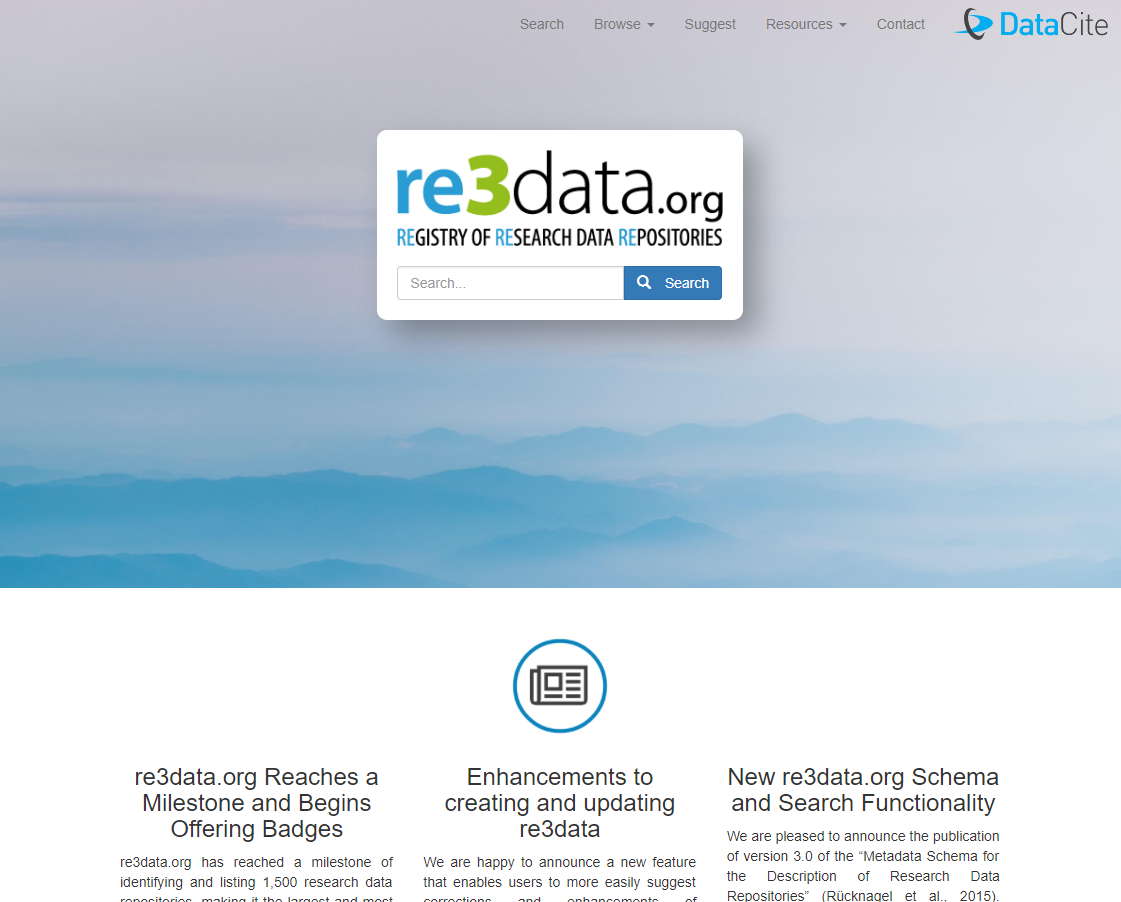
\includegraphics[height=\paperheight]{graphics/re3dataorg.png}};%
		\end{tikzpicture}%
	}%
	\setbeamertemplate{navigation symbols}{}
	\begin{frame}[plain]
	\end{frame}
}

{
	\usebackgroundtemplate{ %
		\begin{tikzpicture}[remember picture, overlay]%
		\node at (current page.center) {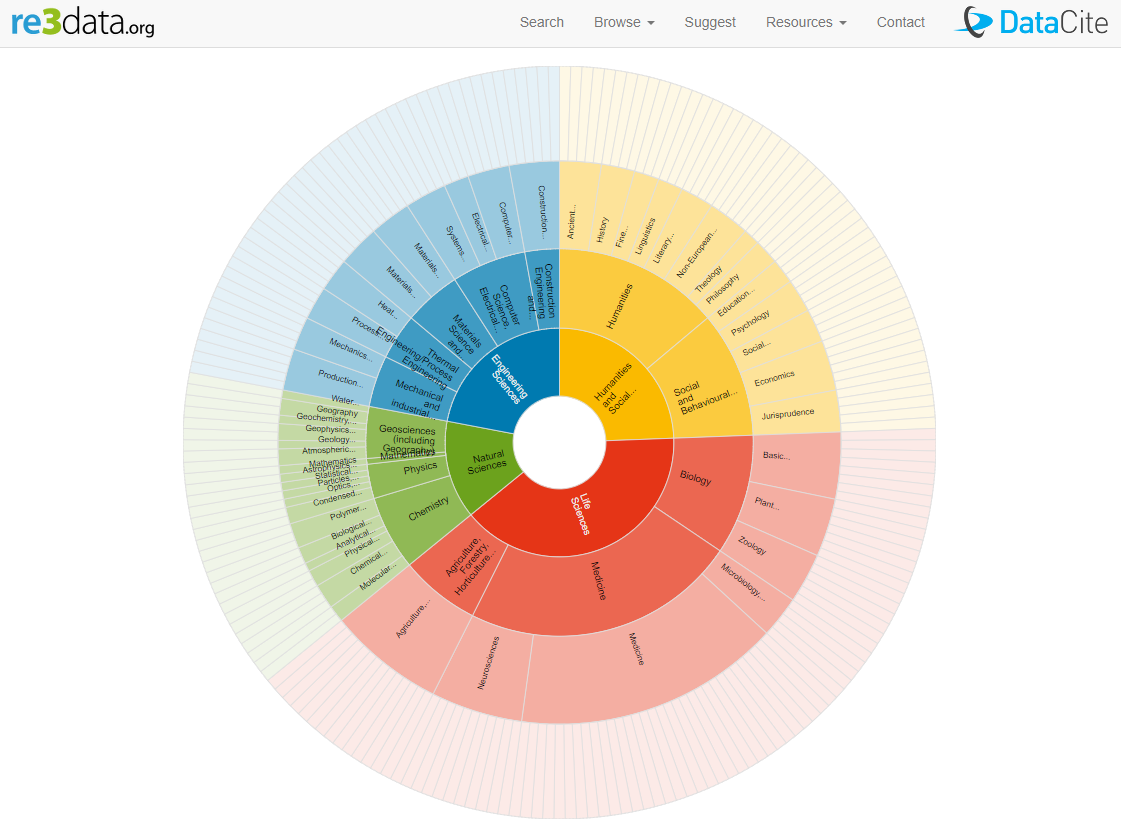
\includegraphics[height=\paperheight]{graphics/re3dataorg-subjects.png}};%
		\end{tikzpicture}%
	}%
	\setbeamertemplate{navigation symbols}{}
	\begin{frame}[plain]
	\end{frame}
}

\begin{frame}
  \frametitle{Retrieve data}
  
  \begin{itemize}
  \item Typically download of one or more files
  \item An API for programmatic retrieval may be available
  \item Data repositories generally support search
  \item Often data are retrieved as they were deposited (original format)
  \item Repository may standardize data during ingestion
  \end{itemize}
\end{frame}

{
	\usebackgroundtemplate{ %
		\begin{tikzpicture}[remember picture, overlay]%
		\node at (current page.center) {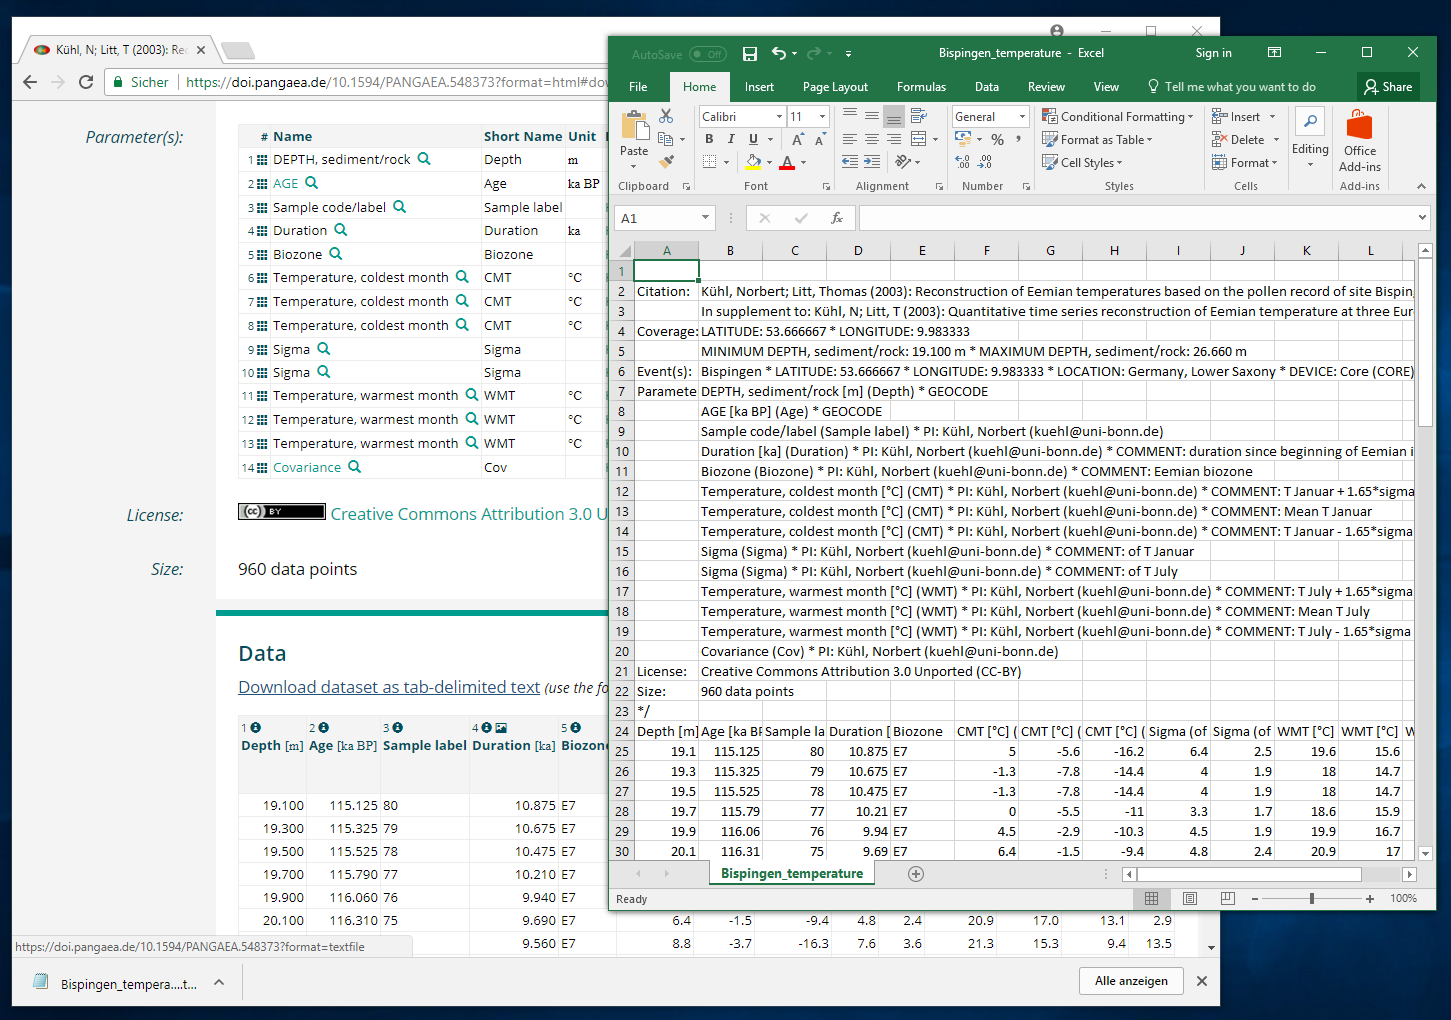
\includegraphics[width=\paperwidth]{graphics/pangaea-download.png}};%
		\end{tikzpicture}%
	}%
	\setbeamertemplate{navigation symbols}{}
	\begin{frame}[plain]
	\end{frame}
}

\begin{frame}
  \frametitle{Reuse data}
  
  \begin{itemize}
  \item Complicated!
  \item Generally substantial processing needed to make reuse possible
  \item Even if accessible, data are generally not interoperable
  \item Little syntactic interoperability due to different formats
  \item Little semantic interoperability due to different terminology
  \item Data quality may not be adequate
  \item Data need to be integrated: common syntax and semantics
  \item A lot of time required to prepare for reuse
  \end{itemize}
\end{frame}

\begin{frame}
  \frametitle{Data Processing}
  
  \begin{itemize}
  \item Assume integrated data
  \item Your next step is to process them for your purpose
  \item Staggering amount of methods
  \item Programming (scripting) languages
  \item Computational environments and other tools
  \end{itemize}
\end{frame}

\begin{frame}
  \frametitle{Curating and storing Data}
  
  \begin{itemize}
  \item As a result of processing, you'll produce new data
  \item Data need to be identified, described, quality controlled, etc.
  \item Curated data are stored and possibly preserved
  \item How you curate and store data depends on various factors
  \item Example factors
  \begin{itemize}
  \item Longevity: from temporary to preserved data
  \item Sharing: with yourself or a community
  \item Dynamism: from static files to queriable databases
  \end{itemize}
  \end{itemize}
\end{frame}

\begin{frame}
  \frametitle{Databases}
  
  \begin{itemize}
  \item
  \end{itemize}
\end{frame}

\begin{frame}
  \frametitle{Versioning and Backup}
\end{frame}

\begin{frame}
  \frametitle{Take aways}
  
\end{frame}

\end{document}
